\documentclass[openany]{book}
% !TeX TXS-program:compile = txs:///pdflatex/[--shell-escape]
\usepackage{macros}
\usepackage{notes}
\usepackage{animate}
\usepackage{paracol}
\usepackage[dvipsnames]{xcolor}
\usetikzlibrary{shapes.geometric}
\usetikzlibrary{calc}
\usepackage{anyfontsize}

\pgfmathsetmacro{\pendulumswing}{40}
\pgfmathsetmacro{\pendulumlength}{5}

%% PICTURES DIRECTORY %%
\graphicspath{{C:/Users/Michael/Pictures/}}

%% REDEFINING CHAPTER FORMATTING %%
\newif\iftoc\titleformat{\chapter}[display]{\cabin}{}{2in}{
	\raggedleft
	\iftoc
	\vspace{2in}
	\else
	{\LARGE\textsc{Week}~{\cantarell\thechapter}} \\
	\fi
	\Huge\scshape\bfseries
}[\vspace{-20pt}\rule{\textwidth}{0.1pt}\vspace{0.0in}]
\titlespacing{\chapter}{0pt}{
	\iftoc
	-100pt+1in
	\else
	-130pt+1in
	\fi
}{0pt}

%% RENEW TITLE PAGE %%
\renewcommand{\mytitle}[2]{%
	\title{#1}
	\author{Michael Pham}
	\date{#2}
	\maketitle
	\newpage
	\mytoc
	\newpage
}

\begin{document}
%\mytitle{Data 100: Principles and Techniques of Data Science}{Spring 2024}
%\pagestyle{empty}

% Background color

\begin{tikzpicture}[remember picture,overlay]
	\fill[BlueViolet] (current page.south west) rectangle (current page.north east);
	
	% Background Hexagon
	\begin{scope}
		\foreach \i in {2.5,...,22}
		{\node[rounded corners,BlueViolet!90,draw,regular polygon,regular polygon sides=6, minimum size=\i cm,ultra thick] at ($(current page.west)+(2.5,-5)$) {} ;}
	\end{scope}
	
	\foreach \i in {0.5,...,22}
	{\node[rounded corners,BlueViolet!90,draw,regular polygon,regular polygon sides=6, minimum size=\i cm,ultra thick] at ($(current page.north west)+(2.5,0)$) {} ;}
	
	\foreach \i in {0.5,...,22}
	{\node[rounded corners,BlueViolet!98,draw,regular polygon,regular polygon sides=6, minimum size=\i cm,ultra thick] at ($(current page.north east)+(0,-9.5)$) {} ;}
	
	\foreach \i in {21,...,6}
	{\node[BlueViolet!95,rounded corners,draw,regular polygon,regular polygon sides=6, minimum size=\i cm,ultra thick] at ($(current page.south east)+(-0.2,-0.45)$) {} ;}
	
	% Course Number
	\node[left,BlueViolet!10,minimum width=0.625*\paperwidth,minimum height=2cm, rounded corners] at ($(current page.north east)+(0,-9.5)$){{\huge Data 100}};
	
	% Title (Line 1)
	\node[left,BlueViolet!5,minimum width=0.625*\paperwidth,minimum height=3cm, rounded corners] at ($(current page.north east)+(0,-11)$){{\fontsize{25}{30} \selectfont \bfseries Principles and Techniques}};
	
	% Title (Line 2)
	\node[left,BlueViolet!5,minimum width=0.625*\paperwidth,minimum height=3cm, rounded corners] at ($(current page.north east)+(0,-12)$){{\fontsize{25}{30} \selectfont \bfseries of Data Science}};
	
	% Name
	\node[left,BlueViolet!5,minimum width=0.625*\paperwidth,minimum height=2cm, rounded corners] at ($(current page.north east)+(0,-14)$){{\Large \textsc{Michael Pham}}};
	
	% Semester	
	\node[rounded corners,fill=BlueViolet!95,text =BlueViolet!5,regular polygon,regular polygon sides=6, minimum size=2.5 cm,inner sep=0,ultra thick] at ($(current page.west)+(2.5,-5)$) {\LARGE \bfseries Sp24};
\end{tikzpicture}

\mytoc

\newpage

\chapter{Introduction to Data Science}
\epigraph{\textit{The purpose of computing is insight,\\not numbers.}}{--- R. Hamming}

\section{Lecture 1 -- 01/16/24}
The course website is located at: \url{https://ds100.org/sp24/}.

\subsection{Course Overview}

\subsubsection{Why Data Science Matters}
Data is used everywhere, from science to sports to medicine. Claims using data also comes up often within discussions (especially about important issues).

Furthermore, Data Science enhances critical thinking. The world is complicated, and decisions are hard. This field fundamentally facilitates decision-making by quantitatively balancing trade-offs.

In order to quantify things reliably, we have to:
\begin{itemize}
	\item Find relevant data;
	\item Recognize the limitations of said data;
	\item Ask the right questions;
	\item Make reasonable assumptions;
	\item Conduct appropriate analysis; and
	\item Synthesize and explain our insights.
\end{itemize}

At each step of this process, we must apply critical thinking and consider how our decisions can affect others.

\newpage

\subsubsection{What is Data Science?}
\begin{defn}[Data Science]\label{def: data science}
	Data Science is the application of data-centric, computational, and inferential thinking to:
	\begin{itemize}
		\item Under the world (science), and
		\item Solve problems (engineering).
	\end{itemize}
\end{defn}

We note that good data analysis is \textbf{not}:
\begin{itemize}
	\item Simple applications of a statistics recipe.
	\item Simple application of software.
\end{itemize}

There are many tools out there for data science, but they are ultimately just tools; we are the ones doing the important thinking.

\subsection{Course Outline}
\subsubsection{Prerequisites}
The official prerequisites are:
\begin{itemize}
	\item \textbf{DATA 8};
	\item \textbf{CS 61A}, DATA C88C, or ENGIN 7; and
	\item EE 16A, \textbf{MATH 54}, or STAT 89A.
\end{itemize}

The bolded course names are the ones that I have already taken.

\subsubsection{Topics (Tentative)}
The tentative list of topics that will be covered in this course is:

\begin{miscbox}{Tentative Topics}
	\begin{multicols}{2}
		\begin{itemize}
			\item Pandas and NumPy
			\item Relational Databases and SQL
			\item Exploratory Data Analysis
			\item Regular Expressions
			\item Visualization
			\begin{itemize}
				\item matplotlib
				\item Seaborn
				\item plotly
			\end{itemize}
			\item Sampling
			\item Probability and random variables
			\item Model design and loss formulation
			\item Linear Regression
			\item Feature Engineering
			\item Regularization, Bias-Variance Tradeoff,\\and Cross-Validation
			\item Gradient Descent
			\item Data Science in the Physical World
			\item Logistic Regression
			\item Clustering
			\item PCA
		\end{itemize}
	\end{multicols}
\end{miscbox}

\subsubsection{Course Components}
With respect to lectures and assignments, the course is structured as follows:
\begin{miscbox}{Course Components}
	\centering
	\begin{center}
		\begin{tabularx}{\textwidth}{Y|Y|Y|Y|Y}
			\textbf{Mo} & \textbf{Tu} & \textbf{We} & \textbf{Th} & \textbf{Fr} \\
			\hline
			& \color{darkgreen}{Live Lecture} & & \color{darkgreen}{Live Lecture} & \\
			\hline
			& \color{darkblue}{Discussion} & \color{darkblue}{Discussion} & & \\
			\hline
			& \color{darkgray}{Office Hours} & \color{darkgray}{Office Hours} & \color{darkgray}{Office Hours} & \color{darkgray}{Office Hours} \\
			\hline
			& & & \color{red}{\textbf{Homework N-1 due}} & \color{darkred}{Homework N released} \\
			\hline
			& \color{red}{\textbf{Lab N-1 due}} & & & \color{darkred}{Lab N released}
		\end{tabularx}
	\end{center}
\end{miscbox}

For lectures, note that there attendance is mandatory; participation will be graded on a 0/1 basis:
\begin{itemize}
	\item Synchronous Participation: complete at least one participation poll question during the live lecture timeslot (11:00am-12:30pm, Tuesdays and Thursdays). As long as you submit a response to at least one poll question in this timeframe, you will receive synchronous attendance credit.
	\item Asynchronous Participation: complete all participation poll questions from the link provided on the course website within one week of the corresponding lecture.
	\item In both cases, participation is graded on completion, not correctness.
\end{itemize}

Also, if we submit all participation polls over the semester, there will be a 0.5\% bonus points applied to the final overall grade.

\subsubsection{Grading}
The grading scheme for this class is as follows:
\begin{miscbox}{Grading Scheme}
	\begin{center}
		\begin{tabularx}{6cm}{X|c}
			\textbf{Category} & \\
			\hline
			Homeworks & 25\% \\
			\hline
			Projects & 10\% \\
			\hline
			Labs & 5\% \\
			\hline
			Discussions & -\\
			\hline
			Lecture Participation & 5\% \\
			\hline
			Midterm Exam & 22.5\% \\
			\hline
			Final Exam & 32.5\% \\
		\end{tabularx}
	\end{center}
\end{miscbox}

\begin{warn}
	\textbf{Important}:
	\begin{itemize}
		\item Midterm: Thursday, March 7, 7-9 PM PST.
		\item Final: Thursday, May 9, 8-11 AM PST.
	\end{itemize}
\end{warn}

\subsection{The Data Science Lifecycle}
The data science lifecycle is a high-level description of the data science workflow. Note in the diagram below that there are two distinct entry points.

\begin{center}
	\begin{animateinline}[controls={play, stop}, controlsaligned = center, loop]{1}
		\multiframe{5}{}{
			% FRAME 1 %
			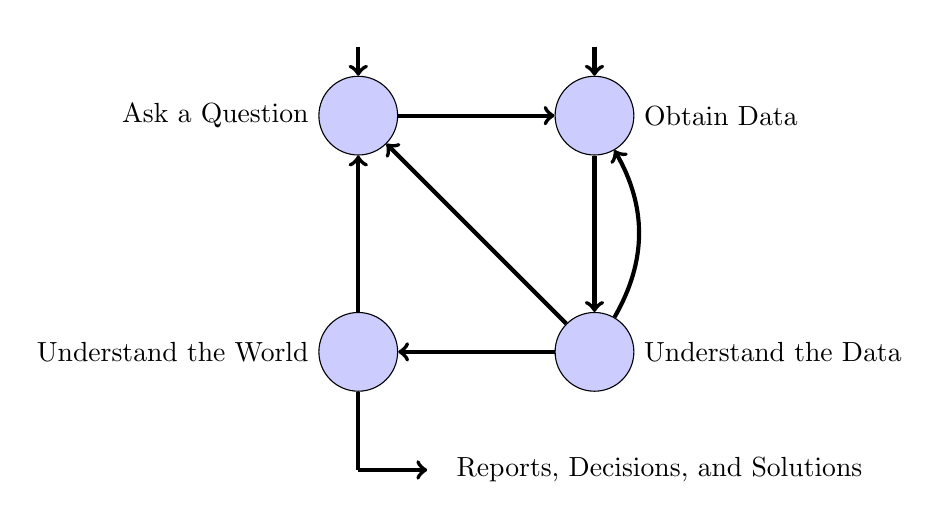
\begin{tikzpicture}
				\node[circle, draw, inner sep = 0pt, minimum width = 1cm, fill = blue!20] at (0,0) (understand_world) {};
				\node[circle, draw, inner sep = 0pt, minimum width = 1cm, fill = blue!20] at (0,3) (ask) {};s
				\node[circle, draw, inner sep = 0pt, minimum width = 1cm, fill = blue!20] at (3,3) (obtain) {};
				\node[circle, draw, inner sep = 0pt, minimum width = 1cm, fill = blue!20] at (3,0) (understand_data) {};
				
				\node at (0,4) (topask) {};
				\node at (3,4) (topobtain) {};
				
				\node at (0,-1.5) (ghostnode) {};
				\node at (1,-1.5) (report) {};
				
				\node[left] at (ask.west){Ask a Question};
				\node[left] at (understand_world.west){Understand the World};
				\node[right] at (obtain.east){Obtain Data};
				\node[right] at (understand_data.east){Understand the Data};
				\node[right] at (report.east){Reports, Decisions, and Solutions};
				
				\draw (understand_world) edge [->, line width = 1.5pt] (ask);
				\draw (understand_data) edge [->, line width = 1.5pt] (understand_world);
				\draw (understand_data) edge [->, line width = 1.5pt] (ask);
				\draw (ask) edge [->, line width = 1.5pt] (obtain);
				\draw (obtain) edge [->, line width = 1.5pt] (understand_data);
				\draw (understand_data) edge[bend right, ->, line width = 1.5pt] node [left] {} (obtain);
				
				\draw (topask) edge [->, line width = 1.5pt] (ask);
				\draw (topobtain) edge [->, line width = 1.5pt] (obtain);
				
				\draw (understand_world) edge [line width = 1.5pt] (ghostnode.center);
				\draw (ghostnode.center) edge [->, line width = 1.5pt] (report);
			\end{tikzpicture}
		
			\newframe
			% FRAME 2 %
			\begin{tikzpicture}
				\node[circle, draw, inner sep = 0pt, minimum width = 1cm, fill = blue!20, opacity = 0.25] at (0,0) (understand_world) {};
				\node[circle, draw, inner sep = 0pt, minimum width = 1cm, fill = blue!20] at (0,3) (ask) {};s
				\node[circle, draw, inner sep = 0pt, minimum width = 1cm, fill = blue!20, opacity = 0.25] at (3,3) (obtain) {};
				\node[circle, draw, inner sep = 0pt, minimum width = 1cm, fill = blue!20, opacity = 0.25] at (3,0) (understand_data) {};
				
				\node at (0,4) (topask) {};
				\node at (3,4) (topobtain) {};
				
				\node at (0,-1.5) (ghostnode) {};
				\node at (1,-1.5) (report) {};
				
				\node[left] at (ask.west){\color{darkblue}{\textbf{Ask a Question}}};
				\node[left, opacity = 0.25] at (understand_world.west){Understand the World};
				\node[right, opacity = 0.25] at (obtain.east){Obtain Data};
				\node[right, opacity = 0.25] at (understand_data.east){Understand the Data};
				\node[right, opacity = 0.25] at (report.east){Reports, Decisions, and Solutions};
				
				\draw (understand_world) edge [->, line width = 1.5pt] (ask);
				\draw (understand_data) edge [->, line width = 1.5pt, opacity = 0.25] (understand_world);
				\draw (understand_data) edge [->, line width = 1.5pt] (ask);
				\draw (ask) edge [->, line width = 1.5pt] (obtain);
				\draw (obtain) edge [->, line width = 1.5pt, opacity = 0.25] (understand_data);
				\draw (understand_data) edge[bend right, ->, line width = 1.5pt, opacity = 0.25] node [left] {} (obtain);
				
				\draw (topask) edge [->, line width = 1.5pt] (ask);
				\draw (topobtain) edge [->, line width = 1.5pt, opacity = 0.25] (obtain);
				
				\draw (understand_world) edge [line width = 1.5pt, opacity = 0.25] (ghostnode.center);
				\draw (ghostnode.center) edge [->, line width = 1.5pt, opacity = 0.25] (report);
			\end{tikzpicture}
		
			\newframe
			% FRAME 3 %
			\begin{tikzpicture}
				\node[circle, draw, inner sep = 0pt, minimum width = 1cm, fill = blue!20, opacity = 0.25] at (0,0) (understand_world) {};
				\node[circle, draw, inner sep = 0pt, minimum width = 1cm, fill = blue!20, opacity = 0.25] at (0,3) (ask) {};s
				\node[circle, draw, inner sep = 0pt, minimum width = 1cm, fill = blue!20] at (3,3) (obtain) {};
				\node[circle, draw, inner sep = 0pt, minimum width = 1cm, fill = blue!20, opacity = 0.25] at (3,0) (understand_data) {};
				
				\node at (0,4) (topask) {};
				\node at (3,4) (topobtain) {};
				
				\node at (0,-1.5) (ghostnode) {};
				\node at (1,-1.5) (report) {};
				
				\node[left, opacity = 0.25] at (ask.west){Ask a Question};
				\node[left, opacity = 0.25] at (understand_world.west){Understand the World};
				\node[right] at (obtain.east){\color{darkblue}{\textbf{Obtain Data}}};
				\node[right, opacity = 0.25] at (understand_data.east){Understand the Data};
				\node[right, opacity = 0.25] at (report.east){Reports, Decisions, and Solutions};
				
				\draw (understand_world) edge [->, line width = 1.5pt, opacity = 0.25] (ask);
				\draw (understand_data) edge [->, line width = 1.5pt, opacity = 0.25] (understand_world);
				\draw (understand_data) edge [->, line width = 1.5pt, opacity = 0.25] (ask);
				\draw (ask) edge [->, line width = 1.5pt] (obtain);
				\draw (obtain) edge [->, line width = 1.5pt] (understand_data);
				\draw (understand_data) edge[bend right, ->, line width = 1.5pt] node [left] {} (obtain);
				
				\draw (topask) edge [->, line width = 1.5pt, opacity = 0.25] (ask);
				\draw (topobtain) edge [->, line width = 1.5pt] (obtain);
				
				\draw (understand_world) edge [line width = 1.5pt, opacity = 0.25] (ghostnode.center);
				\draw (ghostnode.center) edge [->, line width = 1.5pt, opacity = 0.25] (report);
			\end{tikzpicture}
		
			\newframe
			% FRAME 4 %
			\begin{tikzpicture}
				\node[circle, draw, inner sep = 0pt, minimum width = 1cm, fill = blue!20, opacity = 0.25] at (0,0) (understand_world) {};
				\node[circle, draw, inner sep = 0pt, minimum width = 1cm, fill = blue!20, opacity = 0.25] at (0,3) (ask) {};s
				\node[circle, draw, inner sep = 0pt, minimum width = 1cm, fill = blue!20, opacity = 0.25] at (3,3) (obtain) {};
				\node[circle, draw, inner sep = 0pt, minimum width = 1cm, fill = blue!20] at (3,0) (understand_data) {};
				
				\node at (0,4) (topask) {};
				\node at (3,4) (topobtain) {};
				
				\node at (0,-1.5) (ghostnode) {};
				\node at (1,-1.5) (report) {};
				
				\node[left, opacity = 0.25] at (ask.west){Ask a Question};
				\node[left, opacity = 0.25] at (understand_world.west){Understand the World};
				\node[right, opacity = 0.25] at (obtain.east){Obtain Data};
				\node[right] at (understand_data.east){\color{darkblue}{\textbf{Understand the Data}}};
				\node[right, opacity = 0.25] at (report.east){Reports, Decisions, and Solutions};
				
				\draw (understand_world) edge [->, line width = 1.5pt, opacity = 0.25] (ask);
				\draw (understand_data) edge [->, line width = 1.5pt] (understand_world);
				\draw (understand_data) edge [->, line width = 1.5pt] (ask);
				\draw (ask) edge [->, line width = 1.5pt, opacity = 0.25] (obtain);
				\draw (obtain) edge [->, line width = 1.5pt] (understand_data);
				\draw (understand_data) edge[bend right, ->, line width = 1.5pt] node [left] {} (obtain);
				
				\draw (topask) edge [->, line width = 1.5pt, opacity = 0.25] (ask);
				\draw (topobtain) edge [->, line width = 1.5pt, opacity = 0.25] (obtain);
				
				\draw (understand_world) edge [line width = 1.5pt, opacity = 0.25] (ghostnode.center);
				\draw (ghostnode.center) edge [->, line width = 1.5pt, opacity = 0.25] (report);
			\end{tikzpicture}
		
			\newframe
			% FRAME 5 %
			\begin{tikzpicture}
				\node[circle, draw, inner sep = 0pt, minimum width = 1cm, fill = blue!20] at (0,0) (understand_world) {};
				\node[circle, draw, inner sep = 0pt, minimum width = 1cm, fill = blue!20, opacity = 0.25] at (0,3) (ask) {};s
				\node[circle, draw, inner sep = 0pt, minimum width = 1cm, fill = blue!20, opacity = 0.25] at (3,3) (obtain) {};
				\node[circle, draw, inner sep = 0pt, minimum width = 1cm, fill = blue!20, opacity = 0.25] at (3,0) (understand_data) {};
				
				\node at (0,4) (topask) {};
				\node at (3,4) (topobtain) {};
				
				\node at (0,-1.5) (ghostnode) {};
				\node at (1,-1.5) (report) {};
				
				\node[left, opacity = 0.25] at (ask.west){Ask a Question};
				\node[left] at (understand_world.west){\color{darkblue}{\textbf{Understand the World}}};
				\node[right, opacity = 0.25] at (obtain.east){Obtain Data};
				\node[right, opacity = 0.25] at (understand_data.east){Understand the Data};
				\node[right] at (report.east){Reports, Decisions, and Solutions};
				
				\draw (understand_world) edge [->, line width = 1.5pt] (ask);
				\draw (understand_data) edge [->, line width = 1.5pt] (understand_world);
				\draw (understand_data) edge [->, line width = 1.5pt, opacity = 0.25] (ask);
				\draw (ask) edge [->, line width = 1.5pt, opacity = 0.25] (obtain);
				\draw (obtain) edge [->, line width = 1.5pt, opacity = 0.25] (understand_data);
				\draw (understand_data) edge[bend right, ->, line width = 1.5pt, opacity = 0.25] node [left] {} (obtain);
				
				\draw (topask) edge [->, line width = 1.5pt, opacity = 0.25] (ask);
				\draw (topobtain) edge [->, line width = 1.5pt, opacity = 0.25] (obtain);
				
				\draw (understand_world) edge [line width = 1.5pt] (ghostnode.center);
				\draw (ghostnode.center) edge [->, line width = 1.5pt] (report);
			\end{tikzpicture}
		}
	\end{animateinline}
\end{center}

The Data Science Lifecycle goes as follows:
\begin{enumerate}
	\item \textbf{Question/Problem Formulation}
	\begin{itemize}
		\item What do we want to know?
		\item What problems are we trying to solve?
		\item What hypotheses do we want to test?
		\item What are our metrics for success?
	\end{itemize}
	\item \textbf{Data Acquisition and Cleaning}
	\begin{itemize}
		\item What data do we have and what data do we need?
		\item How will we sample more data?
		\item Is our data representative of the population we want to study?
	\end{itemize}
	\item \textbf{Exploratory Data Analysis and Visualization}
	\begin{itemize}
		\item How is our data organized, and what does it contain?
		\item Do we already have the relevant data?
		\item What are the biases, anomalies, or other issues with the data?
		\item How do we transform the data to enable effective analysis?
	\end{itemize}
	\item \textbf{Prediction and Inference}
	\begin{itemize}
		\item What does the data say about the world?
		\item Does it answer our questions or accurately solve the problem?
		\item How robust are our conclusions and can we trust the predictions?
	\end{itemize}
\end{enumerate}

\section{Lecture 2 -- 01/18/24}
\subsection{Tabular Data}
Tabular data simply refers to data that is in a table, where each row represents one observation and each column representing some characteristic, or feature, of the observation.

In this class, we will be using the Python \mylib{\texttt{pandas}} library.
\begin{figurebox}{\texttt{pandas} logo.}
	\centering\includegraphics[height = 2cm]{pandas.png}
\end{figurebox}

With Pandas, we can accomplish a lot of things. Below are a list of some things we will be learning to use Pandas for in this course:
\begin{itemize}
	\item Arranging data in a tabular format.
	\item Extract useful information filtered by specific conditions.
	\item Operate on data to gain new insights.
	\item Apply \mylib{\texttt{NumPy}} functions to our data.
	\item Perform vectorized computations to speed up our analysis.
\end{itemize}

\subsection{DataFrames and Series}
\begin{defn}[DataFrames]\label{def: DataFrames}
	In the language of \texttt{pandas}, we refer to a table as a \texttt{DataFrame}, which is a collection of named columns called \texttt{Series}.
\end{defn}

\begin{defn}[Series]\label{def: Series}
	A \texttt{Series} is a one-dimensional array-like object. It contains:
	\begin{itemize}
		\item A sequence of \texttt{values} of the same type.
		\item A sequence of data labels, called the index.
	\end{itemize}
\end{defn}

\subsubsection{The Series Object}
First, we look at some basic details about the \texttt{Series} object.

\begin{code}{python}{\texttt{Series} Basics}
import pandas as pd

# Creating a Series object
s = pd.Series(["Welcome", "to", "data 100"])
s.index # RangeIndex(start=0, stop=3, step=1)
s.values # array(['welcome', 'to', 'data 100'], dtype='object')
\end{code}

We see that the \texttt{Series} object has \texttt{index} and \texttt{values} variables. Note that we can in fact set custom indices, as shown below:

\begin{code}{python}{Custom Indexing}
# Creating Series with custom indexing
s = pd.Series([-1, 10, 2], index = ["a", "b", "c"])
s.index # Index(['a', 'b', 'c'], dtype='object')

# Changing Series' index
s.index = ["first", "second", "third"]
s.index # Index(['first', 'second', 'third'], dtype='object')
\end{code}

Finally, we can also select a single value or a set of values in a \texttt{Series} object using:
\begin{itemize}
	\item A single label.
	\item A list of labels.
	\item A filtering condition.
\end{itemize}

\begin{code}{python}{Selection}
# Creating a Series
s = pd.Series([4, -2, 0, 6], index = ["a", "b", "c", "d"])

# Selection
s["a"] # Single Label: [4]
s[["a", "c"]] # List of Labels: [4, 0]
s[s > 0] # Filtering Condition: [4, 6]
\end{code}

Note that for selection via filtering condition, we do the following:
\begin{enumerate}
	\item Apply a boolean condition to the \texttt{Series} that satisfy a particular condition.
	\item Index into our \texttt{Series} using this boolean condition. \texttt{pandas} will select only the entries in the \texttt{Series} that satisfy the condition.
\end{enumerate}

\subsubsection{DataFrames}
Typically, we imagine \texttt{Series} as columns within a \texttt{DataFrame} object.

One way to think of a \texttt{DataFrame} is a collection of \texttt{Series} object which shares the same index.

\begin{figurebox}{Relation between \texttt{DataFrame} and \texttt{Series}}
	\centering\includegraphics[height=3.5cm]{dataframe1.png}
\end{figurebox}

The syntax for creating a \texttt{DataFrame} is \inlinecode{\mintinline{python}{pandas.DataFrame(data, index, columns)}}.

We have many approaches for creating a \texttt{DataFrame}. Below are some of the most common ones:
\begin{itemize}
	\item From a CSV file.
	\item Using a list and column name(s).
	\item From a dictionary.
	\item From a \texttt{Series}.
\end{itemize}

\begin{code}{python}{Creating \texttt{DataFrame} Objects}
# From a CSV File
elections = pd.read_csv("data/elections.csv")

# We can also create a DataFrame with one of the columns as the index value
elections = pd.read_csv("data/elections.csv", index_col="Year")

# From a list and column name(s)
pd.DataFrame([1, 2, 3], columns=["Numbers"]) # One column
pd.DataFrame([[1, "one"], [2, "two"]], columns = ["Number", "Description"]) # Multiple columns

# From a dictionary
pd.DataFrame({"Fruit":["Strawberry", "Orange"], "Price": [5.49, 3.99]}) # Specify columns of the DataFrame
pd.DataFrame([{"Fruit":"Strawberry", "Price":5.49}, {"Fruit":"Orange", "Price":3.99}]) # Specify the rows of the DataFrame

# From a Series
s_a = pd.Series(["a1", "a2", "a3"], index = ["r1", "r2", "r3"])
s_b = pd.Series(["b1", "b2", "b3"], index = ["r1", "r2", "r3"])

pd.DataFrame({"A-column":s_a, "B-column":s_b})
\end{code}

\begin{warn}
	Note that indices are not necessarily row numbers! We can set non-numeric values to be the index as well. Furthermore, they aren't necessarily unique either; we can have duplicate values in the index. 
\end{warn}

For example, suppose we ran the following code: 

\begin{center}
	\inlinecode{\mintinline{python}{elections = pd.read_csv("data/elections.csv", index_col = "Candidate")}}
\end{center}

Then, we will get the following \texttt{DataFrame}:
\begin{figurebox}{\texttt{DataFrame} with non-numeric, non-unique indexing.}
	\centering\includegraphics[scale=0.5]{dataframe2}
\end{figurebox}

After creating a \texttt{DataFrame}, we can then change its index using \inlinecode{\mintinline{python}{df.set_index(column_name)}}. And if we happen to change our mind, we can simply do \inlinecode{\mintinline{python}{df.reset_index()}}.

However, while indexes are not necessarily unique, column names in \texttt{pandas} are almost always unique. Having two columns share a name is also just bad practice in general.

We can also extract basic, useful information about a \texttt{DataFrame}, such as its index, columns, and shape.

\begin{code}{python}{Getting Basic \texttt{DataFrame} Information}
# Getting the row labels
elections.index

# Getting the column labels
elections.columns

# Getting the shape of the DataFrame, given in the form (row, col)
elections.shape
\end{code}

\subsection{Data Extraction}
When dealing with data, we want to be able to extract information that we want to work with specifically. Common ways we may want our data is as follows:
\begin{itemize}
	\item Grab the first or last \texttt{n} rows in the \texttt{DataFrame}.
	\item Grab data with a certain label.
	\item Grab data at a certain position. 
\end{itemize}

\subsubsection{.head and .tail}
The simplest scenarios: We want to extract the first or last \texttt{n} rows from the \texttt{DataFrame}.
\begin{itemize}
	\item \inlinecode{\mintinline{python}{df.head(n)}} will return the first \texttt{n} rows of the DataFrame \texttt{df}.
	\item \inlinecode{\mintinline{python}{df.tail(n)}} will return the last \texttt{n} rows.
\end{itemize}

\subsubsection{Label-based Extraction (.loc)}
Something more complex is extracting data with specific columns or index labels. One way to do this is with \inlinecode{\mintinline{python}{.loc}}, which has the following format:
\begin{center}
	\inlinecode{\mintinline{python}{df.loc[row_labels, column_labels]}}
\end{center}

The \inlinecode{\mintinline{python}{.loc}} accessor lets us specify the labels of rows/columns we want to extract. These are the bolded values in a DataFrame.

Arguments to \inlinecode{\mintinline{python}{.loc}} can be:
\begin{itemize}
	\item A list.
	\item A slice.
	\item A single value.
\end{itemize}
\begin{warn}
	Note that for \inlinecode{\mintinline{python}{.loc}}, the slice is, unlike normal Python syntax, \textbf{inclusive} of the right side.
\end{warn}

\begin{code}{python}{Extraction with \texttt{.loc}}
	# Using a list
	elections.loc[[87, 25, 179], ["Year", "Candidate", "Result"]]
	
	# Using a slice
	elections.loc[[87, 25, 179], "Popular vote":"%"]
	elections.loc[:, ["Year", "Candidate", "Result"]] # Gets all rows
	elections.loc[[87, 25, 179], :] # Gets all columns
	
	# Using a single value.
	elections.loc[[87, 25, 179], "Popular vote"] # Note that this returns the Popular vote series, with only the select indices
	elections.loc[0, "Candidate"] # This returns the string value at index 0 from the Candidate column
\end{code}

\begin{figurebox}{\texttt{.loc} using a list.}
	\centering\includegraphics[scale=0.75]{dataframe3}
\end{figurebox}

\begin{figurebox}{\texttt{.loc} using a slice.}
	\centering\includegraphics[scale=0.75]{dataframe4}
\end{figurebox}

\subsubsection{Integer-based Extraction (.iloc)}
A different scenario: We want to extract data according to its position.

To do this, we use \inlinecode{\mintinline{python}{.iloc}}, which allows us to specify the integers of rows and columns we wish to extract. It has the following format:
\begin{center}
	\inlinecode{\mintinline{python}{df.iloc[row_integers, column_integers]}}
\end{center}

Arguments to \inlinecode{\mintinline{python}{.iloc}} can be:
\begin{itemize}
	\item A list.
	\item A slice.
	\item A single value.
\end{itemize}
\begin{warn}
	Note that while the slice was \textbf{inclusive} of the right side for \inlinecode{\mintinline{python}{.loc}}, it is \textbf{exclusive} for \inlinecode{\mintinline{python}{.iloc}}...! Very confusing!!
\end{warn}

The syntax for \inlinecode{\mintinline{python}{.iloc}} is identical to \inlinecode{\mintinline{python}{.loc}}.

\subsubsection{.loc versus .iloc}
While \inlinecode{\mintinline{python}{.loc}} is both safer (i.e. if the order of the data gets shuffled around, our code will still work) and more readable (people actually know what columns we want), \inlinecode{\mintinline{python}{.iloc}} can still be useful!

\begin{example}[Using \texttt{.iloc}]
	If we have a \texttt{DataFrame} of movie earnings sorted by earnings, we can use \inlinecode{\mintinline{python}{.iloc}} to get the median earnings for a given year by indexing into the middle.
\end{example}

\subsubsection{Context-dependent Extraction ([])}
Finally, we have the possibly most-complicated way of extracting data: context-dependent extraction.

\texttt{[]} only takes one argument, which may be:
\begin{itemize}
	\item A slice of row integers.
	\item A list of column labels.
	\item A single column label.
\end{itemize}

\begin{code}{python}{Extraction with \texttt{[]}}
# Using a slice of row integers
elections[3:7]

# Using a list of column labels
elections[["Year", "Candidate", "Result"]]

# Using a single column label
elections["Candidate"]
\end{code}

Using \texttt{[]} is a lot more concise than either \texttt{.loc} or \texttt{.iloc}, hence it's often used more in practice than the other extraction methods.

\chapter{Pandas, and more Pandas!}
\epigraph{\textit{You're as soft as Po,\\the Kung Fu Panda!}}{--- Z. Sherwin}

\section{Lecture 3 -- 01/23/24}
\subsection{Conditional Selection}
We can extract rows that satisfy a given condition. Note that \inlinecode{\mintinline{python}{.loc}} and \texttt{[]} also accept boolean arrays as input; using this, only rows that correspond to \texttt{True} will be extracted.

For example, consider the following code:
\begin{code}{python}{Conditional Selection}
# Getting first ten rows
babynames_first_10_rows = babynames.loc[:9, :]

# Selection with []
babynames_first_10_rows[[True, False, True, False, True, False, True, False, True, False]]

# Selection with .loc
babynames_first_10_rows.loc[[True, False, True, False, True, False, True, False, True, False], :]
\end{code}

In both cases, the following DataFrame will be returned:
\begin{figurebox}{\texttt{DataFrame} with filtered rows.}
	\centering\includegraphics[scale=0.5]{dataframe5}
\end{figurebox}

Using this, we can then extend it to more powerful conditional selections; for example, we can select only rows that are female, \textit{or} were born before 2000 in the DataFrame (or both!):
\begin{center}
	\inlinecode{\mintinline{python}{babynames[(babynames["Sex"] == "F") | (babynames["Year"] < 2000)]}}
\end{center}

This example above also shows us how we can use bitwise operators with our conditionals.

\begin{miscbox}{Bitwise Operators}
	If $p$ and $q$ are boolean arrays or \texttt{Series}, then:
	\begin{center}
		\begin{tabularx}{\textwidth}{|Y|Y|Y|}
			\hline
			\textbf{Symbol} & \textbf{Usage} & \textbf{Meaning} \\
			\hline
			$\sim$ & $\sim p$ & Negation of $p$ \\
			\hline
			$\mid$ & $p \mid q$ & $p$ or $q$ \\
			\hline
			$\&$ & $p \mathbin{\&} q$ & $p$ and $q$ \\
			\hline
			$\mathbin{\char`\^}$ & $p \mathbin{\char`\^} q$ & $p$ xor $q$ \\
			\hline
		\end{tabularx}
	\end{center}
\end{miscbox}

While boolean array selection is useful, it can make our code overly verbose for more complicated conditions. Luckily, \texttt{pandas} offers many alternatives:
\begin{itemize}
	\item \inlinecode{\mintinline{python}{.isin}}
	\item \inlinecode{\mintinline{python}{.str.startswith}}
	\item \inlinecode{\mintinline{python}{.groupby.filter}}
\end{itemize}

\begin{code}{python}{Using \texttt{.isin}}
names = ["Bella", "Alex", "Narges", "Lisa"]

# .isin
babynames[babynames["Name"].isin(names)] # Returns a Series whose entry is True if the corresponding name in babynames is found in the names list

# .str.startswith
babynames[babynames["Name"].str.startswith("N")] # Returns a Series whose entry is True if the corresponding name starts with N
\end{code}

\subsection{Adding, Removing, and Modifying Columns}
\subsubsection{Adding and Modifying Columns}
To add a column, we proceed as follows:
\begin{enumerate}
	\item Use \texttt{[]} to reference the desired new column.
	\item Assign this column to a Series or array of the appropriate length.
\end{enumerate}

We can also modify a column's name or values. The latter's steps are similar to adding a column. For the former, we can use the \inlinecode{\mintinline{python}{.rename()}} function which takes in a dictionary mapping old column names to the new one.

Below, we show how to add, then modify a column:

\begin{code}{python}{Adding and Modifying Columns}
# Create a Series of the length of each name
babyname_lengths = babynames["Name"].str.len()

# Add a column named "name_lengths" that includes the length of each name
babynames["name_lengths"] = babyname_lengths

# Modify the "name_lengths" column to be one less than its original value
babynames["name_lengths"] = babynames["name_lengths"]-1

# Rename "name_lengths" to "Length"
babynames = babynames.rename(columns={"name_lengths":"Length"})
\end{code}

\subsubsection{Removing Columns}
Removing columns a bit more tricky. First, if we want to drop a column, we can use \inlinecode{\mintinline{python}{.drop()}}.

\begin{warn}
	Note that \inlinecode{\mintinline{python}{.drop()}} assumes that we're dropping a row by default; to drop columns, we have to use \inlinecode{\mintinline{python}{axis = "columns"}}...!
	
	Furthermore, we \textbf{must} reassign to the updated DataFrame after dropping a row/column. By default, \texttt{pandas} methods create a copy of the DataFrame, without changing the original DataFrame at all. To apply our changes, we must update our DataFrame to this new, modified copy.
\end{warn}

\begin{code}{python}{Removing Columns}
# Does NOT modify babynames DataFrame
babynames.drop("Length", axis="columns")

# Does modify babynames (through reassignment)
babynames = babynames.drop("Length", axis="columns")
\end{code}

\subsection{Useful Utility Functions}
As stated previously, one of the libraries which we will use is \texttt{NumPy}, which has a lot of useful operations such as \inlinecode{\mintinline{python}{np.mean()}} and \inlinecode{\mintinline{python}{np.max()}}.

And with the \texttt{pandas} library, we have access to a wider array of useful functions. Some which will be covered in this lecture are:
\begin{itemize}
	\item \inlinecode{\mintinline{python}{.shape}}: returns the shape of a \texttt{DataFrame} or \texttt{Series} in the form (rows, cols).
	\item \inlinecode{\mintinline{python}{.size}}: returns the total number of entries in a \texttt{DataFrame} or \texttt{Series}.
	\item \inlinecode{\mintinline{python}{.describe()}}: returns a ``description" of a \texttt{DataFrame} or \texttt{Series} that lists summary statistics of the data.
	\begin{itemize}
		\item For \texttt{DataFrame}: count, mean, std, min/max, quartiles.
		\item For \texttt{Series}: count, unique, top, freq
	\end{itemize}
	\item \inlinecode{\mintinline{python}{.sample()}}: samples a random selection of rows from a \texttt{DataFrame}.
	\begin{itemize}
		\item By default, it is without replacement. Use \inlinecode{\mintinline{python}{replace=True}} for replacement.
		\item Naturally, can be chained with other methods and operators.
	\end{itemize}
	\item \inlinecode{\mintinline{python}{.value_counts()}}: counts the number of occurrences of each unique value in a \texttt{Series}.
	\item \inlinecode{\mintinline{python}{.unique()}}: returns an array of every unique value in a \texttt{Series}.
	\item \inlinecode{\mintinline{python}{.sort_values()}}: sort a \texttt{DataFrame} (or \texttt{Series}).
	\begin{itemize}
		\item \inlinecode{\mintinline{python}{Series.sort_values()}} will automatically sort all values in the \texttt{Series}.
		\item \inlinecode{\mintinline{python}{DataFrame.sort_values(column_name)}} must specify the name of the column to be used for sorting.
	\end{itemize}
\end{itemize}
\begin{warn}
	Note that for \inlinecode{\mintinline{python}{.sort_values()}}, rows are sorted in ascending order.
	
	We can do \inlinecode{\mintinline{python}{.sort_values(ascending=False)}} to sort in descending order.
\end{warn}

\subsubsection{Custom Sorting}
Suppose that we wanted to sort using some custom sorting system. To accomplish this task, there are three main ways of doing so:
\begin{enumerate}
	\item Creating a temporary column and sort Based on the new column.
	\item Sorting using the \texttt{key} argument.
	\item Sorting using the \texttt{map} function.
\end{enumerate}
\begin{code}{python}{Custom Sorting}
# Create a Series of the length of each name
babyname_lengths = babynames["Name"].str.len()

# Approach 1: Create a temporary column
babynames["name_lengths"] = babyname_lengths # Add a column named "name_lengths" that includes the length of each name
babynames = babynames.sort_values(by="name_lengths", ascending=False)

# Approach 2: Sorting using the key Argument
babynames.sort_values("Name", key=lambda x: x.str.len(), ascending=False)

# Approach 3: Sorting using the map Function
def dr_ea_count(string):
  return string.count('dr') + string.count('ea')

babynames["dr_ea_count"] = babynames["Name"].map(dr_ea_count) # Use map to apply dr_ea_count to each name in the "Name" column
babynames = babynames.sort_values(by="dr_ea_count", ascending=False)
\end{code}

\section{Lecture 4 -- 01/25/24}
\subsection{Grouping}
Our goal:
\begin{itemize}
	\item Group together rows that fall under the same category. 
	\begin{itemize}
		\item For example, group together all rows from the same year.
	\end{itemize}
	\item Perform an operation that aggregates across all rows in the category. 
	\begin{itemize}
		\item For example, sum up the total number of babies born in that year.
	\end{itemize}
\end{itemize}

Grouping is a powerful tool as we can perform large operations all at once, and summarize trends within our dataset.

\subsubsection{Group Basics}
To do this, we can use the \inlinecode{\mintinline{python}{.groupby()}} operation, which involves splitting a DataFrame up, applying a function, and then combining the result.

When we call \inlinecode{\mintinline{python}{.groupby()}} on a DataFrame, it generates \texttt{DataFrameGroupBy} objects; these are like sub-frames which contains all rows corresponding to the same group.

When using \inlinecode{\mintinline{python}{.groupby()}}, note that we can't directly work with the \texttt{DataFrameGroupBy} objects; instead, we use some aggregation function with \inlinecode{\mintinline{python}{.agg()}} to transform them back into a \texttt{DataFrame}.

The general syntax for the \inlinecode{\mintinline{python}{.groupby()}} function is:
\begin{center}
	\inlinecode{\mintinline{python}{dataframe.groupby(column_name).agg(aggregation_function)}}.
\end{center}

For example, suppose we ran \inlinecode{\mintinline{python}{babynames[["Year", "Count"]].groupby("Year").agg(sum)}}, which returns the total number of babies born each year. The result is shown in the figure below:

\begin{figurebox}{Demonstration of \texttt{.groupby()}.}
	\centering\includegraphics[scale=0.75]{groupby_demo}
\end{figurebox}

\subsubsection{Aggregation Functions}
A number of things can go inside of the \inlinecode{\mintinline{python}{.agg()}} function:
\begin{paracol}{3}
	\texttt{Python} Functions:
	\begin{itemize}
		\item \inlinecode{\mintinline{python}{.agg(sum)}}
		\item \inlinecode{\mintinline{python}{.agg(max)}}
		\item \inlinecode{\mintinline{python}{.agg(min)}}
	\end{itemize}
	\switchcolumn
	\texttt{NumPy} Functions:
	\begin{itemize}
		\item \inlinecode{\mintinline{python}{.agg(np.sum)}}
		\item \inlinecode{\mintinline{python}{.agg(np.max)}}
		\item \inlinecode{\mintinline{python}{.agg(np.min)}}
		\item \inlinecode{\mintinline{python}{.agg(np.mean)}}
	\end{itemize}
	\switchcolumn
	\texttt{pandas} Functions:
	\begin{itemize}
		\item \inlinecode{\mintinline{python}{.agg("sum")}}
		\item \inlinecode{\mintinline{python}{.agg("max")}}
		\item \inlinecode{\mintinline{python}{.agg("min")}}
		\item \inlinecode{\mintinline{python}{.agg("mean")}}
		\item \inlinecode{\mintinline{python}{.agg("first")}}
		\item \inlinecode{\mintinline{python}{.agg("last")}}
	\end{itemize}
\end{paracol}

Now, with this in mind, we show some alternatives to finding the total number of babies born each year:

\begin{code}{python}{Alternatives with \texttt{.groupby()}}
# Approach 1: Using .agg(sum)
babynames[["Year", "Count"]].groupby("Year").agg(sum)

# Approach 2: Using .sum()
babynames.groupby("Year")[["Count"]].sum()

# Approach 3: Using .sum(numeric_only=True)
babynames.groupby("Year").sum(numeric_only=True) 
\end{code}

\begin{casestudy*}{Name Popularity}{}
Suppose that we wanted to find the female baby name which has fallen in popularity the most in California.

For example, the code below gives us the number of Jennifer's that are born in California per year.
\begin{code}{python}{Jennifer's Popularity}
f_babynames = babynames[babynames["Sex"] == "F"]
f_babynames = f_babynames.sort_values(["Year"])
jenn_counts_series = f_babynames[f_babynames["Name"] == "Jennifer"]["Count"]
\end{code}

A line plot of the data is shown below:
\begin{figurebox}[nofloat]{Line plot of Jennifer's born in California per year.}
	\centering\includegraphics[scale=0.75]{jennifer_popularity}
\end{figurebox}

Well, looking at the count, it certainly looks like the name Jennifer has decreased in popularity!

But, how do we actually \textit{define} ``fallen in popularity"...?
\begin{itemize}
	\item To do this, let's create a metric: ``Ratio to Peak" (RTP). This is the ratio of babies born with a given name in 2022 to the maximum number of babies born with that name in any year. 
\end{itemize}

Going back to the Jennifer example, in 1972, we hit peak Jennifer. 6,065 Jennifers were born. In 2022, there were only 114 Jennifer's. So, calculating the RTP, we get:
\begin{equation*}
	114/6065 = 0.018796372629843364
\end{equation*}

So, we can write a function \inlinecode{\mintinline{python}{ratio_to_peak()}}, then use grouping to calculate the RTP of each name:
\begin{code}{python}{Calculating the RTP}
def ratio_to_peak(series):
  return series.iloc[-1] / max(series)

# This WILL error!
f_babynames.groupby("Name").agg(ratio_to_peak) # Applies ratio_to_peak() onto all columns, even Str-type ones!!

# Calculates the RTP. Returns a table with a Year and Count column
rtp_table = f_babynames.groupby("Name")[["Year","Count"]].agg(ratio_to_peak)

# Calculates the RTP. Returns a table with a Count column
rtp_table = f_babynames.groupby("Name")[["Count"]].agg(ratio_to_peak)
rtp_table = rtp_table.rename(columns = {"Count": "Count RTP"}) # Renames Count column to Count RTP

# Finds the top ten lowest RTP names
top10 = rtp_table.sort_values("Count RTP").head(10).index
# Plots the data
px.line(f_babynames[f_babynames["Name"].isin(top10)], x = "Year", y = "Count", color = "Name")
\end{code}

And after running the code above, we see that ``Debra" has fallen in popularity the most out of all the names in California! For a visual representation of the ten names with the lowest RTP, we refer to the following graph:
\begin{figurebox}[nofloat]{Line graph of names which has fallen in popularity the most in California.}
	\centering\includegraphics[scale=0.75]{ten_lowest_rtp}
\end{figurebox}
\end{casestudy*}

All in all, remember that the result of a groupby operation applied to a \texttt{DataFrame} is a \texttt{DataFrameGroupBy} object.

And once we're given a \texttt{DataFrameGroupBy} object, we can use various functions to generate \texttt{DataFrames} (or \texttt{Series}). Note that \inlinecode{\mintinline{python}{.agg()}} is only one choice! Some other options are:

\begin{paracol}{3}
	\begin{itemize}
		\item \inlinecode{\mintinline{python}{df.groupby(col).mean()}}
		\item \inlinecode{\mintinline{python}{df.groupby(col).sum()}}
		\item \inlinecode{\mintinline{python}{df.groupby(col).min()}}
		\item \inlinecode{\mintinline{python}{df.groupby(col).max()}}
	\end{itemize}
	\switchcolumn
	\begin{itemize}
		\item \inlinecode{\mintinline{python}{df.groupby(col).first()}}
		\item \inlinecode{\mintinline{python}{df.groupby(col).last()}}
		\item \inlinecode{\mintinline{python}{df.groupby(col).size()}}
		\item \inlinecode{\mintinline{python}{df.groupby(col).count()}}
	\end{itemize}
	\switchcolumn
	\begin{itemize}
		\item \inlinecode{\mintinline{python}{df.groupby(col).filter()}}
	\end{itemize}
\end{paracol}

See \url{https://pandas.pydata.org/docs/reference/groupby.html} for a list of \texttt{DataFrameGroupBy} methods that we can use!


\subsubsection{groupby.size() versus groupby.count()}
One of the more subtle differences between some functions is that of \inlinecode{\mintinline{python}{.groupby().size()}} and \inlinecode{\mintinline{python}{.groupby().count()}}.

\inlinecode{\mintinline{python}{.size()}} returns a \texttt{Series} object counting the number of rows in each group. This is similar to \inlinecode{\mintinline{python}{.value_counts()}}, though it does not sort the index based on the frequency of entries.

\begin{figurebox}[]{\texttt{groupby.size()} demo.}
	\centering\includegraphics[scale=0.75]{groupby_size}
\end{figurebox}

On the other hand, with \inlinecode{\mintinline{python}{.count()}}, it returns a \texttt{DataFrame} with the counts of non-missing values in each column.

\begin{figurebox}[]{\texttt{groupby.count()} demo.}
	\centering\includegraphics[scale=0.75]{groupby_count}
\end{figurebox}

\subsubsection{Filtering by Groups}
Another common use for groups is to filter data.
\begin{itemize}
	\item \inlinecode{\mintinline{python}{groupby.filter()}} takes an argument \texttt{func}.
	\item \texttt{func} is a function that:
	\begin{itemize}
		\item Takes a DataFrame as input.
		\item Returns either \textcolor{darkgreen}{\texttt{True}} or \textcolor{darkred}{\texttt{False}}.
	\end{itemize}
	\item \texttt{filter} applies \texttt{func} to each group/sub-\texttt{DataFrame}:
	\begin{itemize}
		\item If \texttt{func} returns \textcolor{darkgreen}{\texttt{True}} for a group, then all rows belonging to the group are preserved.
		\item If \texttt{func} returns \textcolor{darkred}{\texttt{False}} for a group, then all rows belonging to that group are filtered out.
	\end{itemize}
\end{itemize}

\begin{warn}
	Some caveats to filtering:
	\begin{itemize}
		\item Filtering is done per group, not per row. This is different from boolean filtering!
		\item Unlike \inlinecode{\mintinline{python}{agg()}}, the column we grouped on does NOT become the index!
	\end{itemize}
\end{warn}

\begin{figurebox}[]{Filtering by groups demo.}
	\centering\includegraphics[scale=0.75]{groupby_filter}
\end{figurebox}
\end{document}